\chapter{Background}

In this section we present an introduction to the GPU architecture and network intrusion detection system (NIDS).

\section{GPU Architecture} 
We have used Tesla K80 cards for our research. It offers GPU programming capability by providing the Compute Unified Device Architecture (CUDA) SDK. The GPU consists of SMs (Streaming Multiprocessors) which consists of SPs(Streaming Processors). In Tesla K80 there are 13 SMs and 192 SPs per SM with Compute Capability 3.7. Every new CUDA specification is given a standard number, which is known as Compute Capability. SPs share the control login and the instruction cache. The global memory of the GPU is formed by the Graphic Double Data Rate (GDDR) DRAM. The global memory of Tesla K80 is 11520 MBytes.

A function which is to be executed on the GPU is known as kernel,which is launched by specifying the total number of threads required to execute it. The total number of threads required per block and the total number of blocks required is specified while launching the kernel. SPs execute the threads and SMs execute one or more thread blocks concurrently. The thread blocks do not migrate to other SMs. 

The thread blocks are divided into warps. A warp consists of 32 threads and all the threads in a warp execute the same instruction. All the threads in a warp execute in SIMD (Single Instruction Multiple Data) mode which means all the threads execute the same instruction but with different data. In Tesla K80 we can assign 2048 threads per SM and 1024 threads per block. Since there are 13 SMs there can be 26624 threads which can be launched.

The SM can choose the warp to execute which has no latency. SMs execute thread blocks and SPs execute threads. If we launch the kernel with 13 thread blocks and 192 threads per thread block, it may not be a good decision, because we need to launch multiple thread blocks per SM to hide the memory latency. The SM can switch to a different warp which has zero latency. This method is known as oversubscription.

There are different types of memories in the GPU. They are global memory, shared memory, constant memory and registers. Shared memory is on-chip and it is faster when compared to the global memory which is off-chip. Tesla K80 has 11.25 GB global memory, 64 KB constant memory, 48 KB shared memory/block and 64K registers/block. 


Global memory can be access by all the threads executing the kernel and the host. Shared memory is shared between all the threads in the thread bock. Each warp consists of 32 warps, thus there are 32 banks in shared memory. Each bank is sectioned into 32 bit words or 4 bytes. Every bank can service only one request per cycle, hence if there are multiple requests to the same bank, it arises to a situation known as bank conflict. When there are no bank conflicts, shared memory is as fast as register memory. Each thread has its own set of registers. The latency to access from registers is 0 cycles when there are no read after write latencies. To hide the read write latency it may take up to 768 threads per thread block. Register pressure can also cause to degrade the performance. Register pressure means there are not enough registers to handle the task. In this case the the data is “spilled over” to the local memory. 

Local memory is off-chip memory and the latency is same as the global memory. The compiler saves the automatic variables in the local memory when there is not enough space in the registers. Large structures are typically stored in Local memory. Thus we can optimize the code by storing the data in shared memory and registers.

CUDA is similar to the C programming language. It has made GPU programming much easier for a developer. The important features it provides are the ability to read and write to the shared memory and the global memory.

\subsection{Network Intrusion Detection System (NIDS)}
Network Intrusion detection systems collect the packets that passes through the network and checks to see if it is legitimate. If it identifies any suspicious activity it either logs it or alerts the network. An example of NIDS is Snort. Snort consists of thousands of signatures and the signatures are applied to the packets flowing across the network to detect malicious activity. There are two types of NIDS, one of them work with signatures and the other employ machine learning to detect anomalies. The examples of signatures are security threats and viruses which will be used to find if they exists in packet’s payload. The drawback of signature based analysis is that for new attacks they are ineffective; they can be effective only after the attack is manually detected and a signature is found. The signatures are patterns which we search in network traffic. 

IDS perform checking of the header as well as searching for the payload if it contains any viruses. Some examples of checking the header can be searching if the IP addresses are in the reserved IP address or checking if we found a malicious TCP flag bit combination. Examples of the patterns in the payload can be finding email containing a virus or DNS buffer overflow attack. The pattern matching algorithms can be classified as single pattern matching or multi pattern matching. With single pattern matching the entire payload is searched only if a single pattern exists. So the time complexity is the product of the number of patterns and the length of the largest pattern. To search for multiple patterns, the same algorithm should be applied to individual patterns. In multi-pattern matching algorithms, Finite state machines are used to build the intermediate states and multiple patterns are searched simultaneously. Hence the run time complexity is independent of the number of patterns and the maximum length of a pattern. According to Zha (2013), “ Snort, on the other hand, because of its use of an efficient multipattern search algorithm has a runtime that is independent of the number of patterns in the dictionary and linear in the length of the target string.” 

\subsection{CUDA Programming Environment}
CUDA C provides an interface for programmers who are familiar with C to develop applications on the GPU. CUDA C provides APIs which allow the programmer to define functions in C which are called as kernel. When kernels are called they are going to be executed N times in parallel by N CUDA threads, unlike the C function which would be executed only once. The GPU threads will be identified using a  one-dimensional,two-dimensional or three-dimensional  thread index, which when grouped together form a  one-dimensional,two-dimensional or three-dimensional  block of threads, which are called a thread block. These thread blocks provide an easy way to invoke the elements of a matrix, or vector to perform computations.

The threads in a thread blocks run on a same processor core and they need to share the memory resources which are limited on that core. Hence there is a limit on the number of threads per thread block, which is either 512 or 1024 on current GPUs if the compute capability of the device is >=2.0. But, the kernel will be executed by multiple thread blocks of equal size, so the total number of threads can be calculated as equal to the number of threads per block multiplied by the number of blocks.

The blocks are grouped together into a one-dimensional,two-dimensional or three-dimensional grid of thread blocks as shown in figure~\ref{fig:cudablock} If the GPU has compute capability >=2.0, then the three dimensional grid of thread blocks is supported. The threads in a thread-block can be  1D, 2D or 3D for all compute capabilities. The size of the grid is decided by the size of the data which it processes or the number of SMs in the device, which can be exceeded.

\begin{figure}
	\centering
	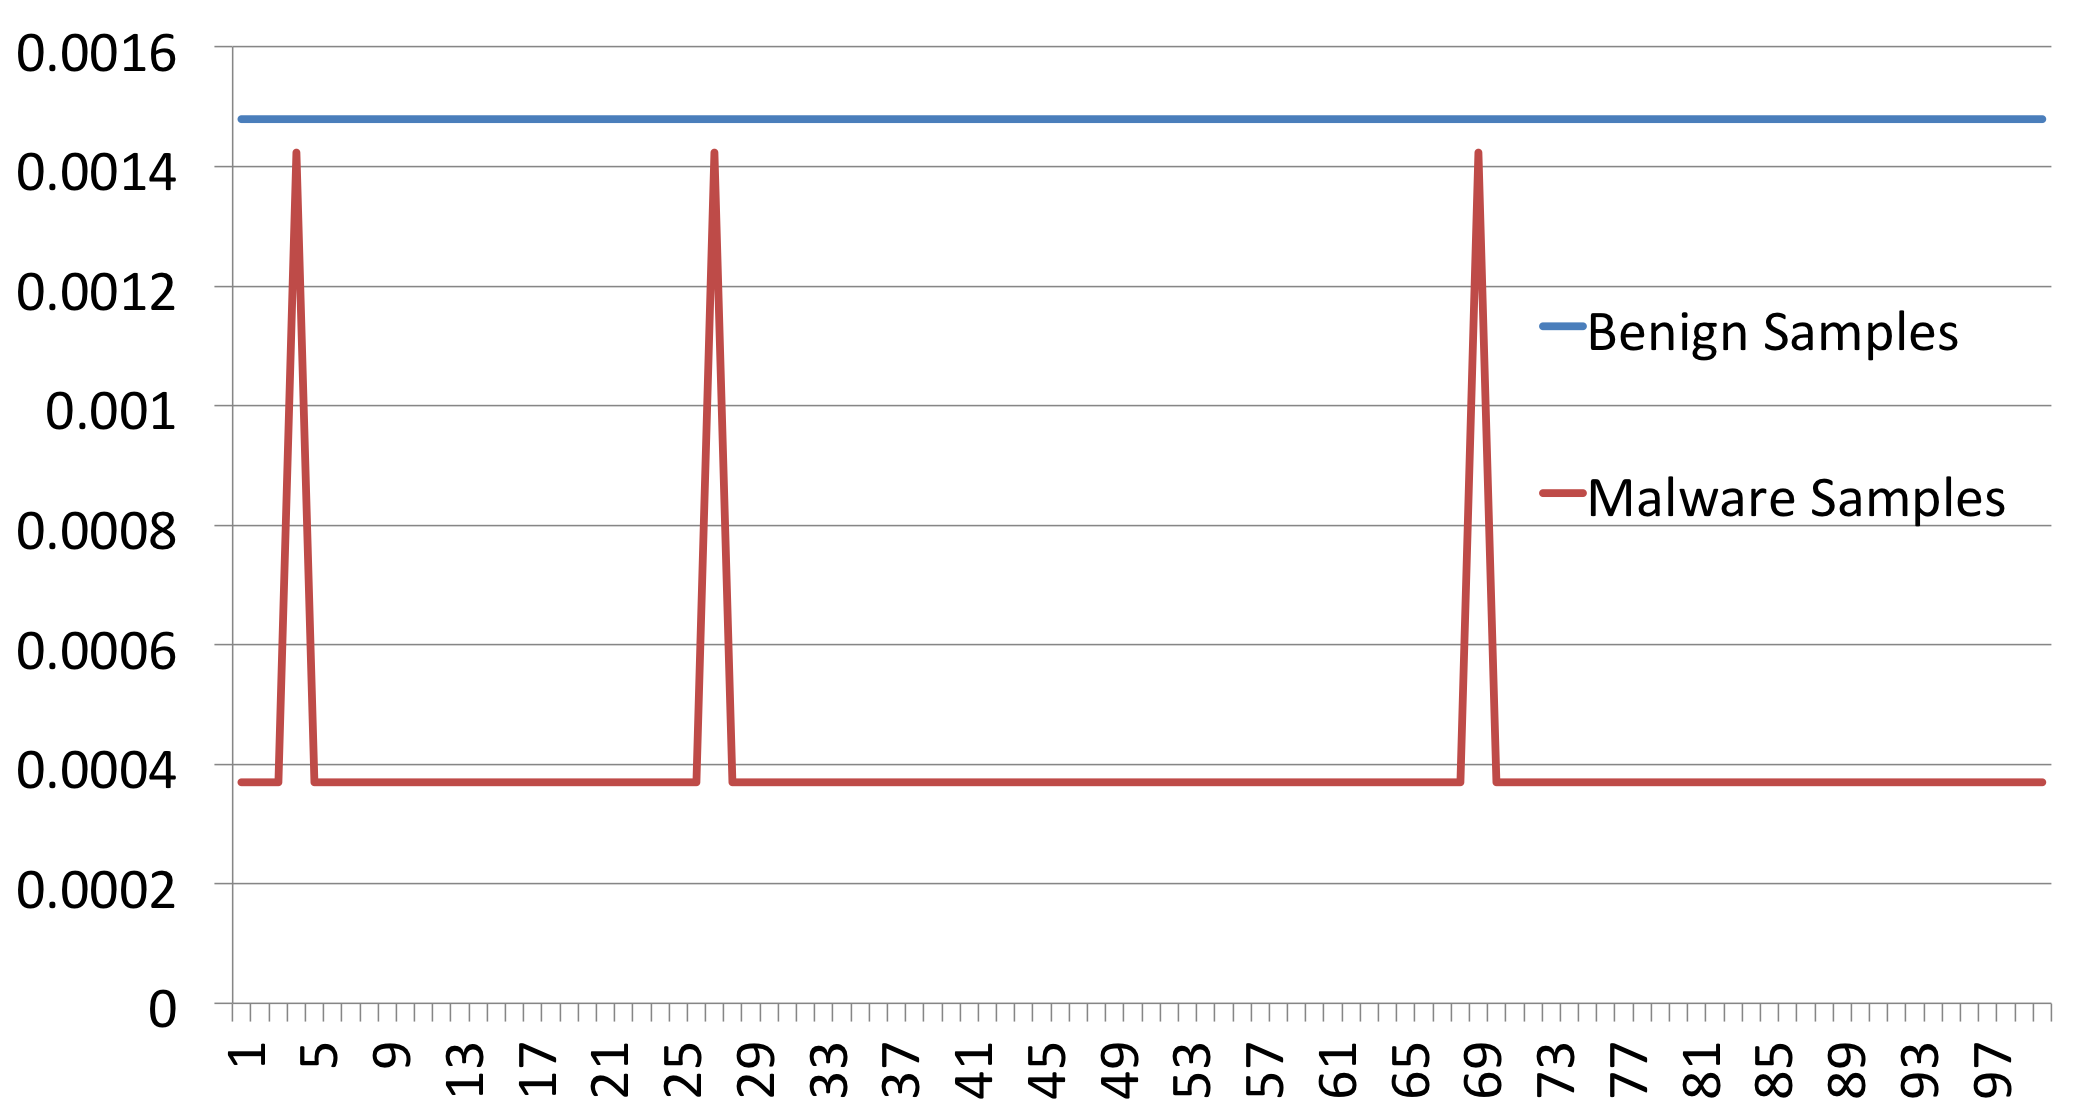
\includegraphics[width=8.4cm, height=10cm]{500.png}
	\caption[Meta-language instructions example]{Meta-language instructions example \cite{bib4}.}
	\label{fig:cudablock}
\end{figure}


\section{CUDA Thread Execution Model} 

The number of blocks in a grid can be found using the built-in variable gridDim and the number of threads in a block can be found using the built-in variable blockDIm. A thread block is indexed by the variable blockIdx and a thread in a thread block is indexed by threadIdx. The variables blockIdx and threadIdx have members which represent the x,y and z components. For a one-dimensional kernel, threadIdx.x is used to uniquely identify a thread within a thread block and blockIdx.x is used to uniquely identify a block within a grid.

\subsection{Synchronizing CUDA Threads}
syncthreads is the barrier for threads in a thread block. Threads can be synchronized only across the threads in a thread block, but not across the threads in a grid, the reason is because CUDA wants to execute the thread blocks on any streaming multiprocessors(SM) in any order. 
The waiting thread blocks can be scheduled on any SM, and there is no need to wait for any thread block to finish execution. This allows CUDA applications to scale well, by improving the performance when there are more SM’s by executing multiple blocks concurrently when compared to platforms with less SM’s. 

\subsection{Assigning CUDA Threads}
During a kernel invocation, the CUDA runtime will assign the thread block to the SM’s in the device. Each SM can be assigned a maximum of eight thread blocks on any platform. The programmer should ensure there are enough registers, shared memory and threads to execute the blocks. If the number of resources are not sufficient, the run time will assign less blocks to the SM. 

The total number of blocks that can be concurrently executed depends on the GPU. The Kepler architecture has a total of 13 streaming multiprocessors (SM’s) which can concurrently handle 16 blocks, which gives a maximum limit of 208 thread blocks.

The Kepler architecture has compute compatibility 3.7 hence we are able to create thread blocks which consists of at most 1024 threads, then the Tesla K80 GPU can support 212,992 threads residing in the SM’s for execution. In the next section, I will describe how the threads are actually scheduled on the SM’s.

\subsection{Scheduling CUDA Threads}
The streaming multiprocessor schedules threads in groups of 32 threads called warp.
Each SM has 4 warp schedulers and 8 instruction dispatch units which allows four warps to be dispatched and executed concurrently. Kepler has a quad-warp scheduler which selects 4 warps and  2 instructions from each warp to be dispatched every cycle. Kepler allows double precision instructions to execute along with other instructions. Fermi did not allow other instructions to execute along with double precision instructions.

One SM consists of 192 SPs (Streaming Processors) - 8 groups of 24 per SM. Each SP (CUDA core) has fully pipelined execution units for floating-point and integer arithmetic operations.

Kepler’s warp scheduler selects two instructions from each warp to be issued to a group of  twenty four cores, four load/store units, or four special function units (SFU’s).

At the most 16 blocks of 1024 threads each can be issued to each SM, which indicates 32 warps can be assigned to each SM. But each clock cycle, only 4 warps out of the 32 warps are scheduled on the SM. The reason is that the instruction in a kernel can take many clock cycles to execute (for example, reading from global memory will need many cycles). An instruction which takes many clock cycles to execute will cause a latency. To hide this latency, instructions from other warps will be issued to the SM while the previous warp is still waiting for the result. This technique is often called latency hiding.

\begin{figure}
	\centering
	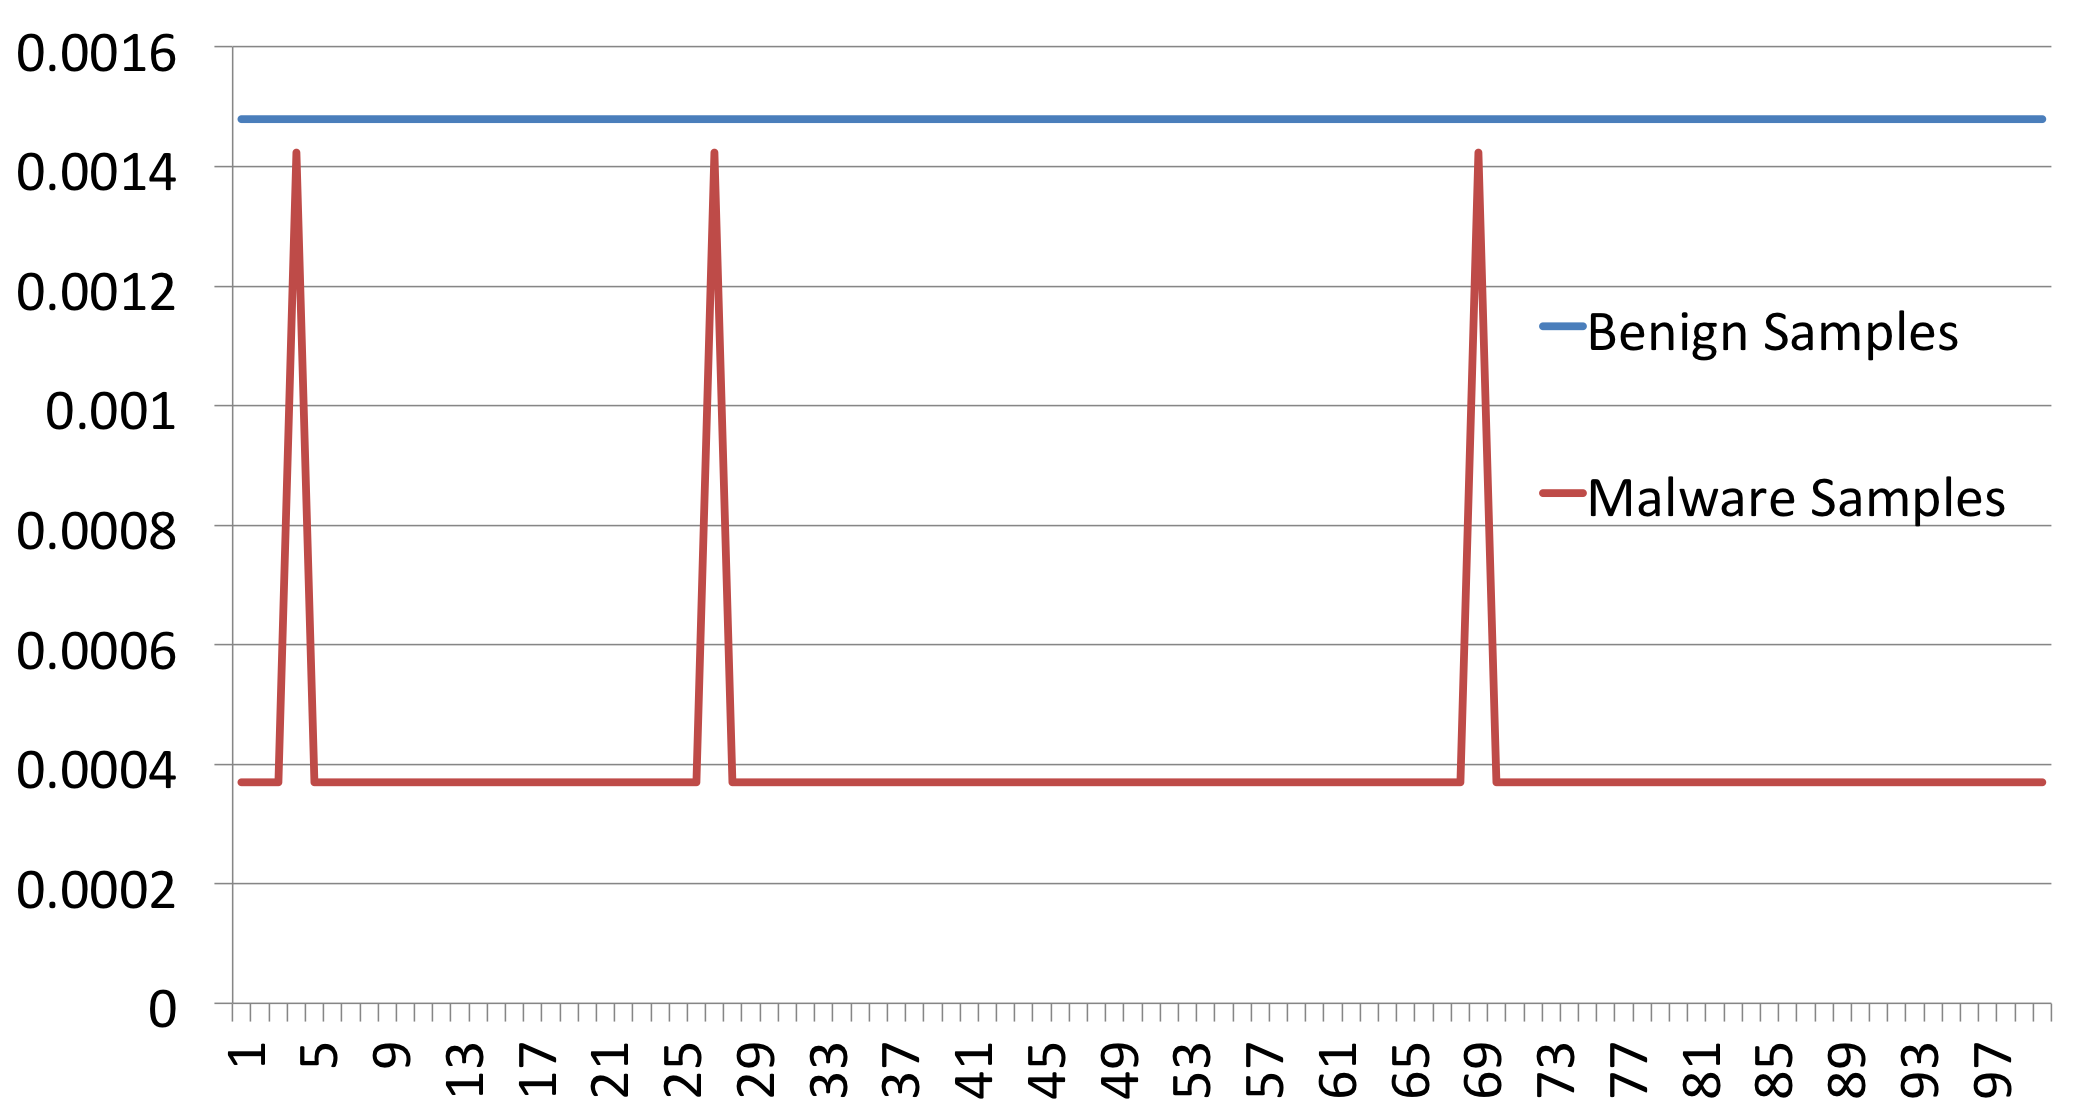
\includegraphics[width=9cm, height=4.5cm]{500.png}
	\caption{A single warp scheduler unit\cite{bib1}.}
	\label{fig:warpscheduler}
\end{figure}

\subsection{Thread Divergence}
Thread divergence is caused due to the branch statements such as if-then-else, switch and loop statements such as for. Divergence can happen only inside a warp. When an if condition evaluates to be true for some threads of the warp, the other threads of  the warp will be disabled. For example, if 8 threads of a warp evaluate to true, then the performance of the warp is reduced to 8/32 * 100 = 25 percent because 16 threads were disabled while evaluating the true condition.
When the threads complete the if condition execution all the threads are enabled again. 

\begin{figure}
	\centering
	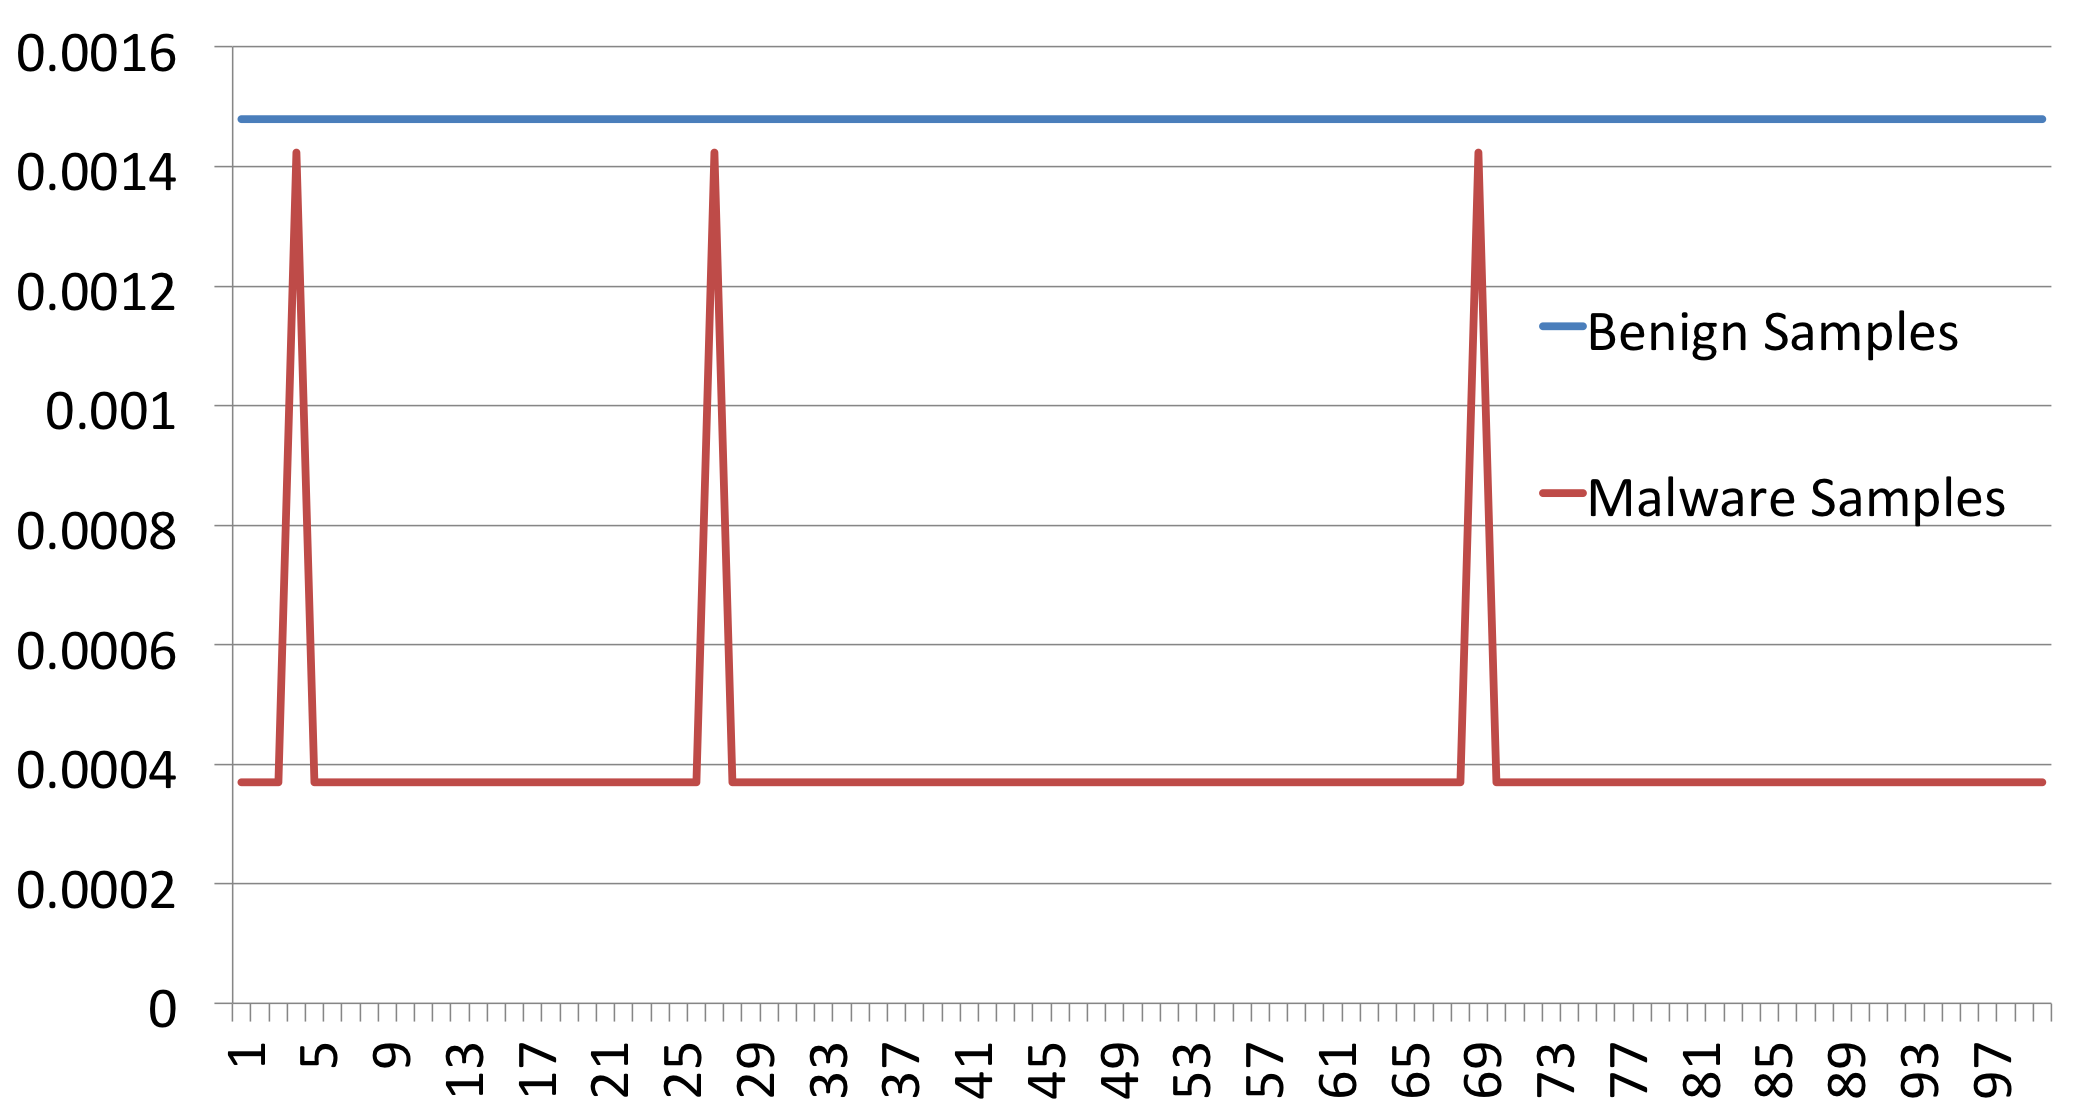
\includegraphics[width=9cm, height=4.5cm]{500.png}
	\caption{A single warp scheduler unit\cite{bib1}.}
	\label{fig:warpdivergence}
\end{figure}

The threads with even numbered index executes PathA and threads with odd numbered index executes PathB.

Since some of the threads take PathA and others take PathB, the total execution time of the warp is the sum of time taken by the threads in PathA and the time taken by the threads in PathB. One way to eliminate warp divergence would be to have all threads in a block to follow the same execution path. Thus, all the threads in a warp follow the same execution path and there would be no warp divergence in a block.

CUDA kernels can be coded using PTX, the instruction set architecture or a high level programming language such as C/C++ which is more effective. In either case the kernel should be compiled by nvcc to generate the binary and the binary can be executed on the GPU. nvcc is the compiler which compiles C or PTX code. 

\subsection{Shared Memory}

Shared memory is divided into n separate banks and if there are n memory requests to n different banks, then the request would be serviced in a single transaction. If the n memory requests are to the same bank, then the transactions are serialized yielding to a decrease in the bandwidth by a factor of n.

For devices of Compute Capability 3.7, the shared memory is split into 32 banks of bandwidth 64 bits per clock cycle. The shared memory can be addressed using two modes which can be configured using cudaDeviceSetSharedMemConfig(). In the default 32 bit mode, consecutive 32 bit words map to successive banks.Shared memory bank conflicts are not generated when two threads of a warp access any sub-word within a 32 bit word or access two 32-bit words whose addresses x and y are in the same 64-bit word segment(address of this segment is a multiple of 64) and y = x + 32(even if the addresses x and y fall in the same bank). In the 64  bit mode, consecutive 64 bit words map to successive banks. Shared memory bank conflicts are not generated when two threads of a warp access any sub-word within a 64-bit word(even if the addresses  fall in the same bank). 

\begin{figure}
	\centering
	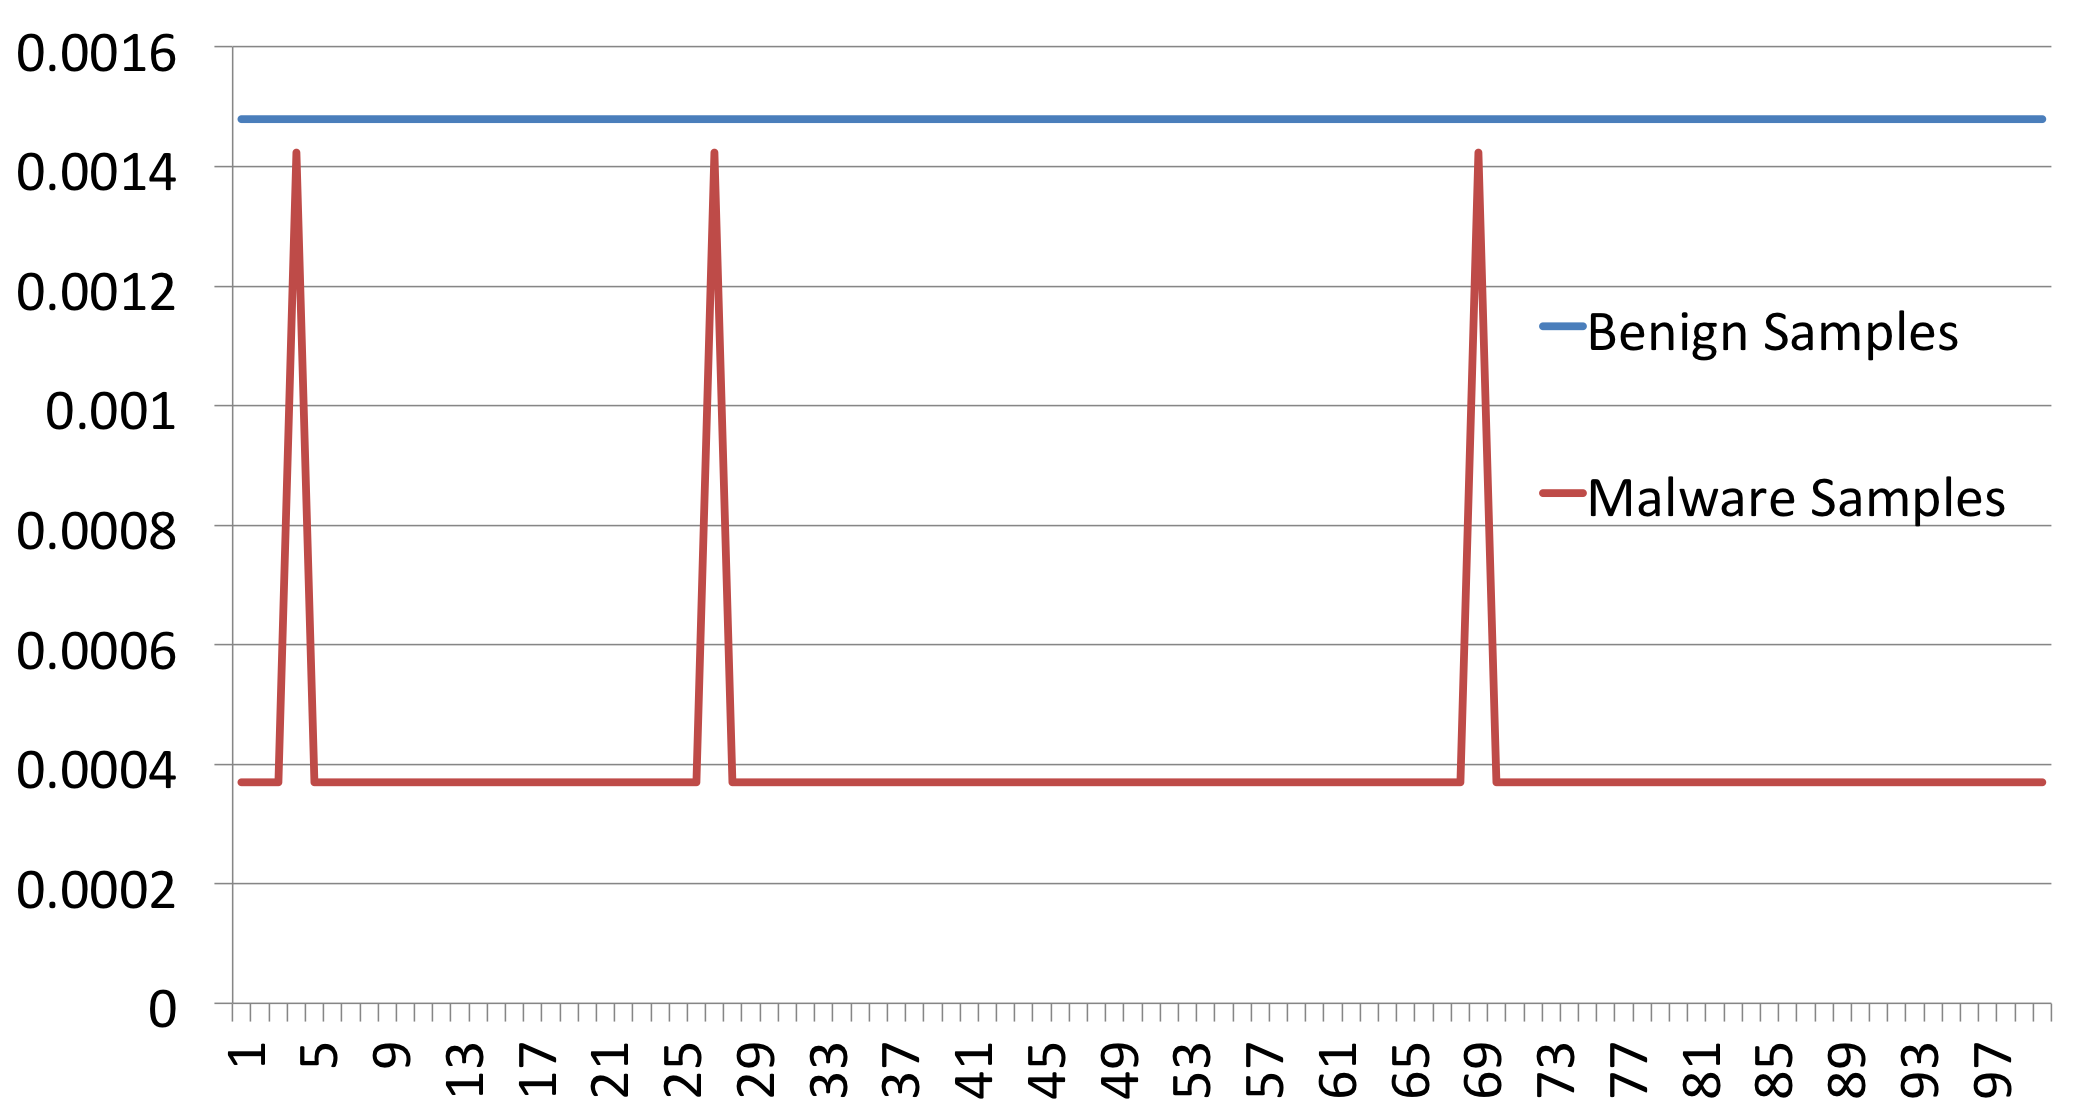
\includegraphics[width=9cm, height=4.5cm]{500.png}
	\caption{Bank conflicts in the four byte addressing mode\cite{bib2}.}
	\label{fig:bankconflicts}
\end{figure}

\subsection{Pinned Memory}
CudaHostAlloc is used to allocate Pinned Memory. Pinned memory can be directly accessed by the device and thus it can be read or written with a higher bandwidth when compared to the pageable host memory. When memory is allocated using malloc the data becomes pageable host memory.

The GPU cannot directly access pageable host memory, the CUDA driver should temporarily allocate a page-locked or pinned memory, copy the data from the host to the pinned memory and then copy the data from the pinned memory to the device memory. From Figure ~\ref{fig:packetpinnedmemory} we can observe that Pinned Memory is used for temporary buffer area when transferring data between CPU and GPU. This can be avoided by directly allocating our host arrays on the Pinned Memory. Pinned Memory can be allocated using cudaHostAlloc() or cudaMallocHost() and de-allocate it with cudaFreeHost().

\begin{figure}
	\centering
	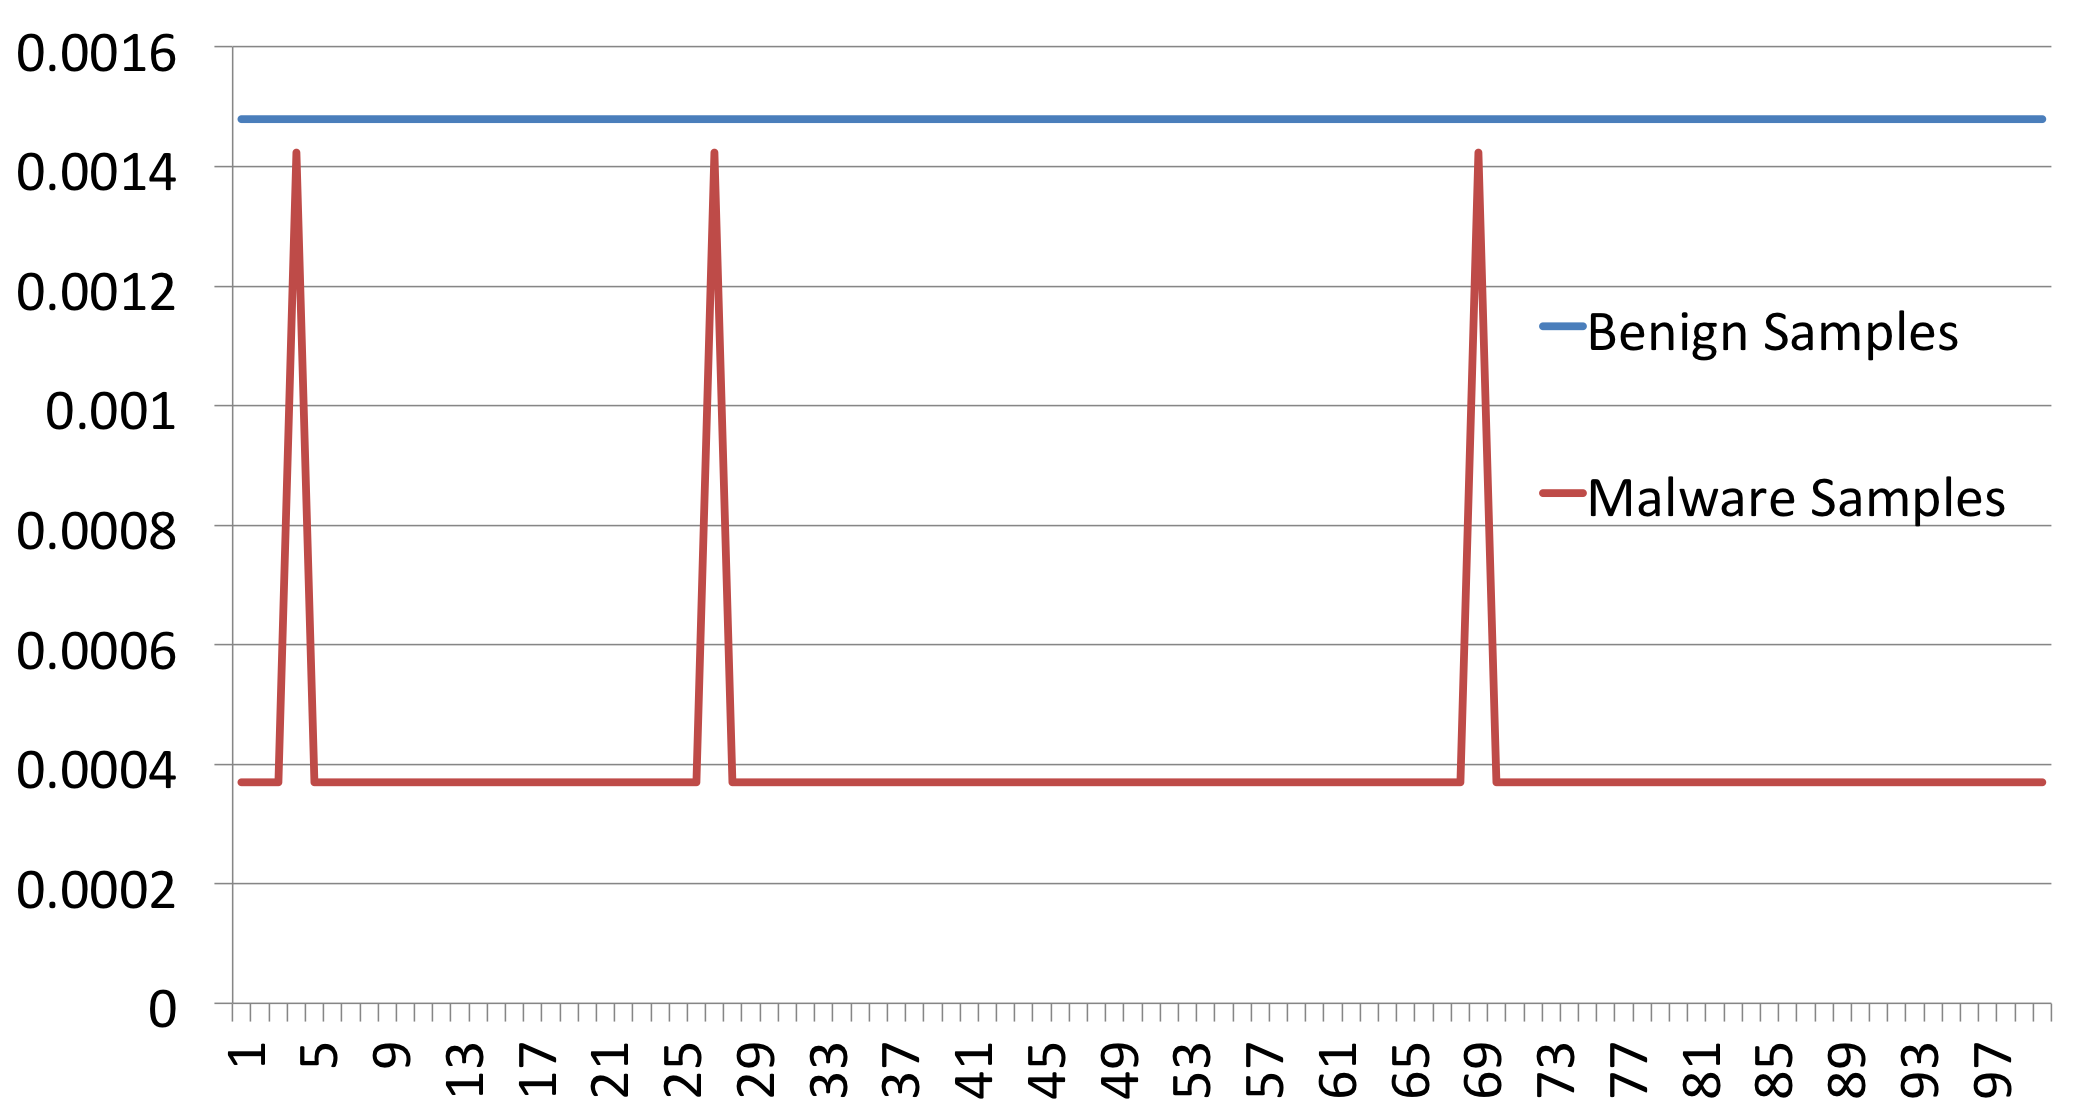
\includegraphics[width=8.4cm, height=10cm]{500.png}
	\caption{Copying data to Pinned Memory \cite{bib3}}
	\label{fig:packetpinnedmemory}
\end{figure}

The global memory, Local Memory, Constant memory and Texture memory are stored in physical DRAM chips which are present surrounding the GPU. The difference between these memories is the way they are cached. As shown in the below fig 3.4. The silver GTX 580 is the GPU and the DRAM chips are the black colored chips surrounding the GPU.


In section 3, the System organization, the parallelism approaches, header checking and pattern matching will be explained.